% -*- TeX-master: "User_guide"; fill-column: 75 -*-

\section{Differences between the class hierarchies}
\label{sec:extended-type-hierarchy}

\begin{sidewaysfigure}[p]
  \centering
  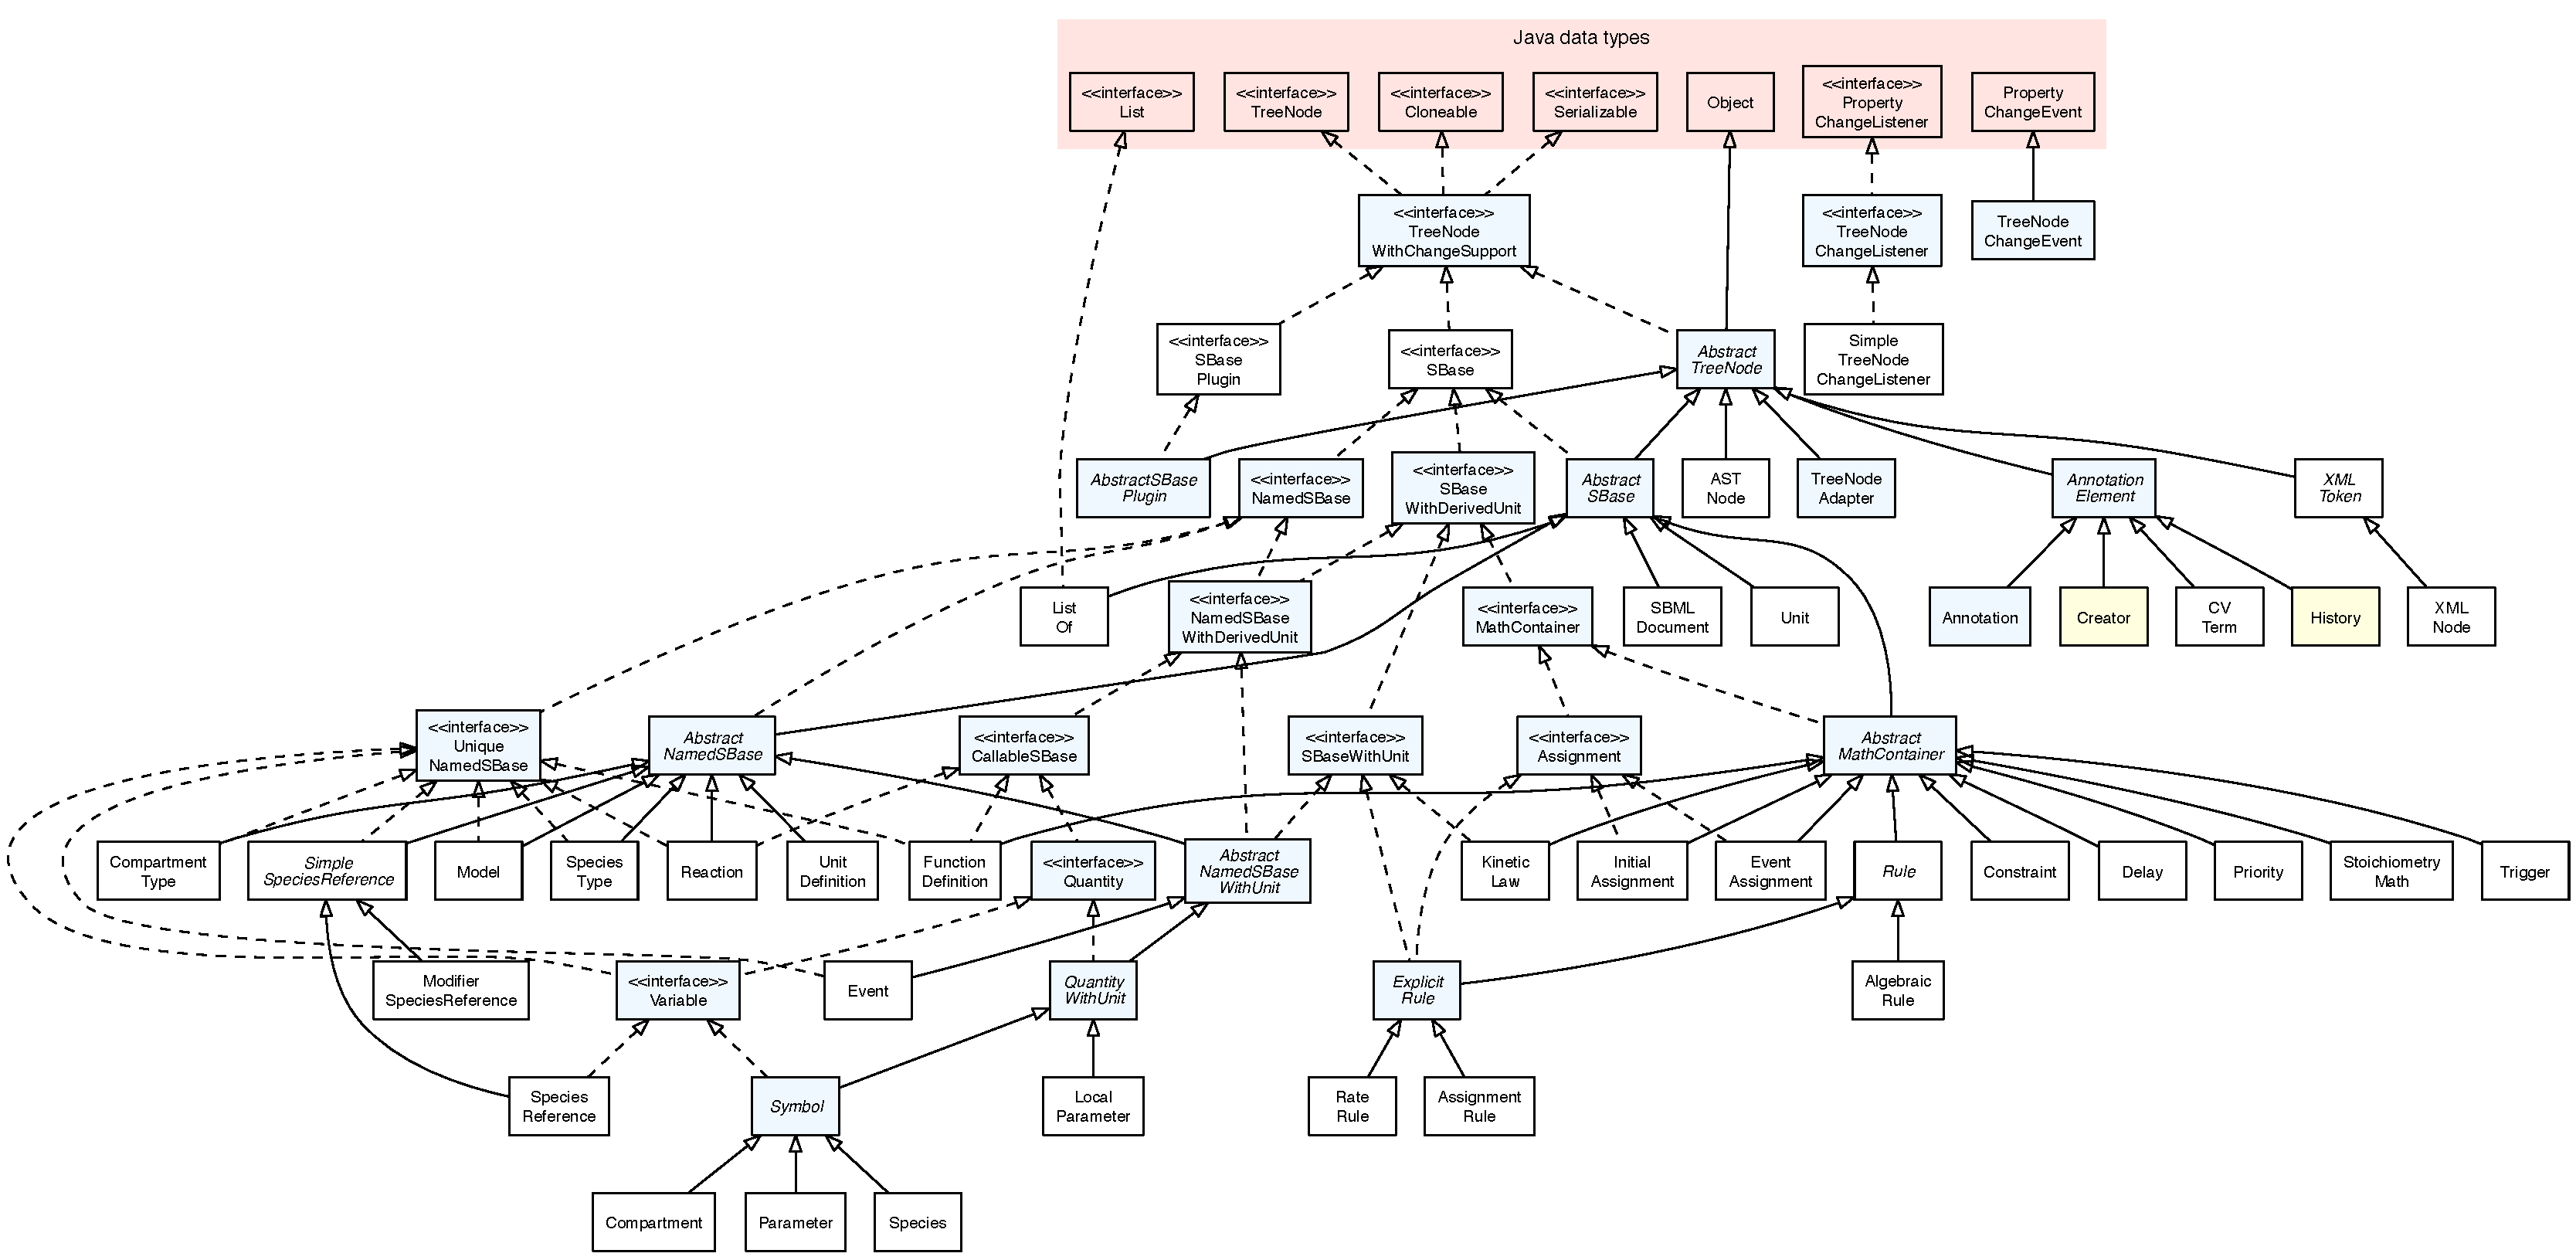
\includegraphics[width=0.97\textwidth]{../common/img/FullTypeHierarchy.pdf}
  \caption[The type hierarchy of the main SBML constructs in JSBML]{The
    type hierarchy of the main SBML constructs in JSBML. The elements
    colored in yellow, \code{Creator} and \code{History}, correspond to
    \code{ModelCreator} and \code{ModelHistory} in libSBML. Elements
    colored in blue are additional, in most cases abstract, data types in
    JSBML that do not have corresponding features in libSBML. Many other
    classes and interfaces in this diagram have no equivalent in libSBML,
    but offer more powerful capabilities for Java programmers. By making
    \SBase extend the interface \TreeNodeWithChangeSupport (another class
    defined by JSBML), which in turn extends the Java interfaces
    \code{Cloneable}, \code{Serializable}, and \TreeNode. All subclasses
    of \code{SBase} also provide the functionality of these classes and
    interfaces. In JSBML, even SBML components that are not defined by
    SBML as actually being derived from \code{SBase} are nevertheless
    derived from \TreeNodeWithChangeSupport; thus, they (and all their
    subclasses) share many common methods and attributes, which makes them
    easy to use when wherever instances of \TreeNode or operations across
    hierarchies of objects are needed. In order to support SBML Level~3
    packages, JSBML version 1.0 adds the interface \SBasePlugin and its
    abstract implementation \AbstractSBasePlugin (shown marked
    with a red border in this diagram).} 
  \label{fig:TypeHierarchy}
\end{sidewaysfigure}

Wherever multiple SBML elements defined in at least one SBML Level/Version
combination \index{SBML!specification} share attributes, JSBML
\index{JSBML!type hierarchy} provides a common superclass or at least a
common interface that gathers methods for manipulating the shared
properties. Consequently, JSBML's type hierarchy
\index{application programming interface!JSBML} is richer than libSBML's (see
\vrefrange{fig:TypeHierarchy}{fig:MathContainerHierarchy}).

Just as in libSBML, \index{application programming interface!libSBML} all
SBML objects derived from SBML's \SBase extend the JSBML abstract class
\SBase, but in JSBML, \SBase is an interface rather than an object class.
This allows more complex relations to be defined between derived data
types. In contrast to libSBML, JSBML's \SBase extends the interface
\TreeNodeWithChangeSupport, which in turn extends three other interfaces:
\Cloneable, \Serializable, and \TreeNode (\fig*{fig:SBase}).
This brings with it various advantages. One is that, because all elements
defined in JSBML \index{cloning} override the \code{clone()} method from
the class \code{java.lang.Object}, \index{Object@\code{Object}} all JSBML
elements can be deeply copied and are therefore \emph{cloneable}. Further,
extending the interface \Serializable makes it possible for JSBML
\index{application programming interface!JSBML} objects to be stored in
binary form without having to write them explicitly to an SBML file.
\index{SBML!XML file} In this way, programs can easily load and save their
in-memory objects or send data structures across a network connection
without the need of additional file encoding and subsequent parsing.

The third interface extended by \SBase, \TreeNode is defined in Java's
\emph{Swing} \index{graphical user interface!Swing} package; however,
\TreeNode is actually independent of any graphical information.  (We hasten
to add that JSBML does \emph{not} depend on any particular graphical user
interface, and no other classes are initialized when loading \TreeNode from
Java Swing.)  \TreeNode defines recursive methods on hierarchically
structured data types, such as iteration over all successors. This means
that, if a developer so desires, all instances of JSBML's \SBase interface
can be passed directly to the Java Swing \index{graphical user
  interface!Swing} class \JTree \index{graphical user
  interface!\code{JTree}} for easy visualization. The program shown in
\fig{fig:JSBMLvisualizer-source} (and whose output is presented in
\fig{fig:JSBMLvisualizer-output}) demonstrates the simple code
needed to parse an SBML file \index{SBML!XML file} and immediately display
its contents in a \JFrame. \index{graphical user interface!\code{JFrame}}
The \ASTNode class in JSBML is also derived from all these three interfaces
and can hence be cloned, serialized, and visualized in the same way.

\begin{figure}[hb]
 \centering
 \vspace*{2ex}
 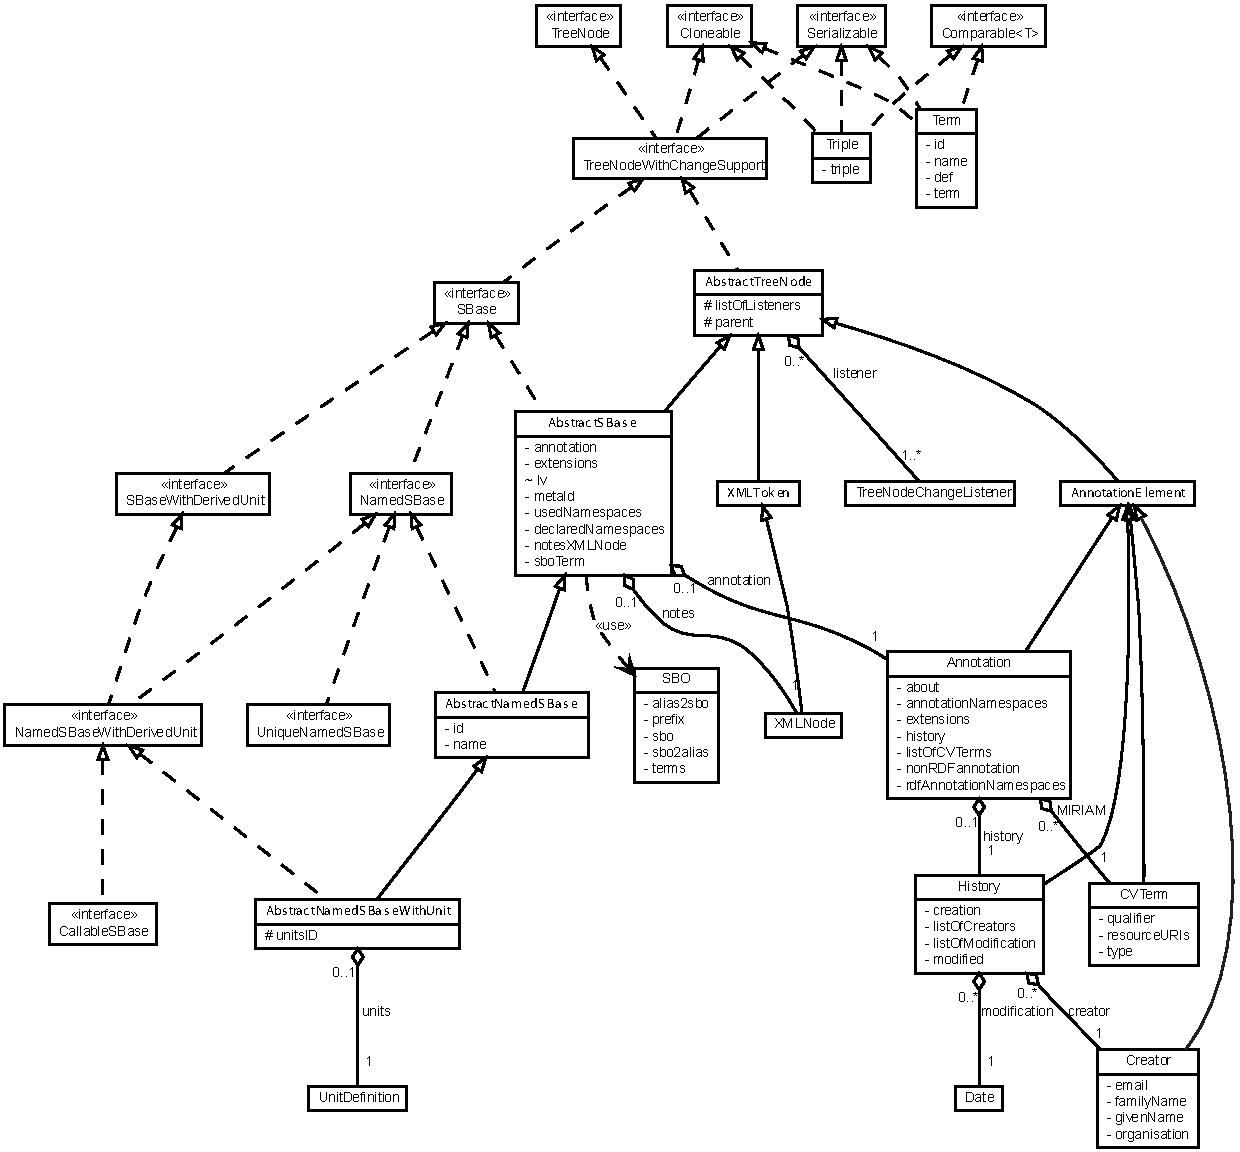
\includegraphics[width=\textwidth]{../common/img/SBase.pdf}
 % SBase.pdf: 1001x568 pixel, 72dpi, 35.31x20.04 cm, bb=0 0 1001 568
 \caption[The interface \code{SBase}]{The interface \SBase. This figure
   shows the most important top-level data structures in JSBML, with a
   focus on the differences compared to libSBML. For the sake of clarity,
   we have omitted all the methods on the classes shown here. As can be
   seen in this diagram, all data types that
   represent SBML constructs in JSBML extend \AbstractTreeNode.
   Derivatives of \SBase extend either one of the two abstract
   classes \AbstractSBase or \AbstractNamedSBase, which in turn
   also extend \AbstractTreeNode. The class \SBO implements
   facilities for parsing the ontology\index{Ontology} file provided on the
   SBO web site (\url{http://www.ebi.ac.uk/sbo/main/}) in OBO format (Open
   Biomedical Ontologies), using a parser provided by the BioJava
   project~\citep{Holland2008}. \SBO stores its ontology in
   the classes \code{Term} that are interrelated in \code{Triples}
   consisting of subject, predicate, and object (each being an instance of
   \code{Term}).}
 \label{fig:SBase}
\end{figure}


\subsection{Common interface for hierarchical structures: \codeNC{AbstractTreeNode}}%
\label{sec:AbstractTreeNode}
\index{TreeNode!AbstractTreeNode@\code{AbstractTreeNode}}

When reading the SBML specifications~\citep{Hucka2003, Hucka2008,
  Hucka2010a}, \index{SBML!specification} it quickly becomes apparent that
an SBML model has a tree-shaped, hierarchical structure, with \SBase being
the superclass of nearly all other SBML components. In JSBML, other kinds of
objects besides \SBase are also organized hierarchically within an
\SBMLDocument.  To unify the programming interfaces for all of these kinds
of objects, JSBML defines abstract data types as top-level ancestors for
its \SBase implementation as well as all other hierarchical elements, such
as \Annotation, \ASTNode, \Creator, \CVTerm, \History, and \XMLNode (for
notes in XHTML \index{XHTML} format).

As mentioned above, the interface \TreeNodeWithChangeSupport defines a
cloneable and serializable version of \TreeNode. (See the diagram in
\fig{fig:SBase}.) In addition, it also provides methods to notify
dedicated \TreeNodeChangeListener class objects about any changes within
the data structure. Its abstract implementation, \AbstractTreeNode,
implements many of the methods inherited from \TreeNodeWithChangeSupport
and also maintains a list of change listeners (implemented as
\TreeNodeChangeListener{}s). Furthermore, this class contains a basic
implementation of the methods \code{equals} and \code{hashCode}, which both
make use of a recursive call over all descendants within the hierarchical
SBML data structure. By basing the object definitions on this class, the
implementation of all derived classes has become much simpler.


\subsection{Common root of SBML components: \codeNC{AbstractSBase}}

With \SBase being an interface rather than an object class, most SBML-related
object classes in JSBML extend the abstract implementation \AbstractSBase, as
shown in \fig{fig:SBase}.  One of the features of this abstract class is
that it tracks the SBML Level and Version of every concrete object
implementing it.  The need for tracking each object's Level+Version
combination individually (a feature shared with libSBML) may seem odd at
first.  The need arises because a software system may need to work with more
than one combination at a given time; it may also need to create individual
SBML components before they are hooked into \SBMLDocument, which again
requires that individual objects know the SBML Level and Version for which
they were created.


\subsection{Interface for SBML components with identifiers: \codeNC{NamedSBase}}

Some classes of objects derived from \SBase in SBML contain an identifier,
colloquially often simply called the \emph{id}. JSBML gathers all elements
that have SBML identifiers under the common interface \NamedSBase. The JSBML
class \AbstractNamedSBase extends \AbstractSBase and implements this
interface.  

The interface \UniqueNamedSBase is shared by those elements whose
identifiers must be unique within the model. The identifiers of all instances
of \NamedSBase that do not implement \UniqueNamedSBase but belong to the same
group, such as all \UnitDefinition instances, must be unique if these identifiers are
defined. The Boolean method \code{isIdMandatory()} on \NamedSBase indicates
if an identifier must be defined for an element in order to create a valid
SBML data structure.  This is required in JSBML because the \Model object
stores direct pointers in the form of a hash from the identifier of the
corresponding object if \code{isIdMandatory()} returns \code{true}. 
The method decides if registering an element for its identifier has been a
success even if no identifier has been defined for this element. It is
necessary to have the method \code{isIdMandatory()}, because even if something
implements \UniqueNamedSBase, the identifier might be optional, as is the
case with \SimpleSpeciesReference. But the \Model class has to decide if and
where to store the identifier-to-element mapping in its hash. For details, see
the \Model class, where you can find some methods named \code{registerIds}, in
which the Boolean method is called.

The only elements with non-unique identifiers are \UnitDefinition, whose
identifiers exist in a separate namespace, and \LocalParameter, whose
identifiers may shadow the identifiers of global elements. (However, within a
given list of \UnitDefinition objects or list of \LocalParameter objects,
duplicate identifiers are not allowed.)

Internally, JSBML only uses the attribute \emph{id} for unique identifiers.
When you work with SBML Level~1, where the SBML specifications only define
name attributes (i.e., no identifiers) for elements, calls to
\code{setName(String)} are redirected to \code{setId(String)}. For all other
SBML Levels, an SBML element's \emph{name} can be specified separately from
the \emph{id} and does not have to be unique. In contrast to the identifier,
there is no syntax check on the name because it can consist of any UTF-8
character. The class that manipulates identifiers and names is
\AbstractNamedSBase; all classes with identifiers and names (optional
or mandatory) are derived from \AbstractNamedSBase. Accordingly,
\code{getName()} returns the identifier if working with SBML Level~1, but
internally it is redirected to \code{getId()}. For all other Levels,
\code{getName()} and \code{getId()} may yield different values, depending on
what is set for the class.

Summarizing, all classes in JSBML that implement the (empty) interface
\UniqueNamedSBase are types of \SBase, more precisely \NamedSBase (interface)
or \AbstractNamedSBase (abstract class), whose identifier must be unique through
the entire SBML model if it is set. \UnitDefinition and \LocalParameter do not
implement this interface. These are {\NamedSBase}s, whose identifier may
override the identifiers of elements that do implement \UniqueNamedSBase, but
not other {\UnitDefinition}s or other {\LocalParameter}s within the same
\KineticLaw. A Level and Version dependent syntax check ensures the validity of
identifiers. In this way, the correctness of the model is ensured and the \Model
class can centrally maintain hashes for elements with identifiers. This
significantly speeds up the getXXX(String id) methods.


\subsection{Interface for SBML components with units: \codeNC{SBaseWithDerivedUnit}}

Many SBML components represent some quantitative value with which a unit of
measurement is associated. However, the numerical value of an SBML
component does not necessarily have to be defined explicitly in the model;
it may instead be determined by a mathematical formula contained in a given
\SBase object in the model.  This implies that the unit associated with the
value may be derivable.  In JSBML, the interface \SBaseWithDerivedUnit is
used to represent all components that either explicitly or implicitly
contain some unit.  \fig{fig:Variable} shows this part of JSBML's
type hierarchy in more detail.

\begin{figure}[b]
  \vspace*{2ex}
  \centering
  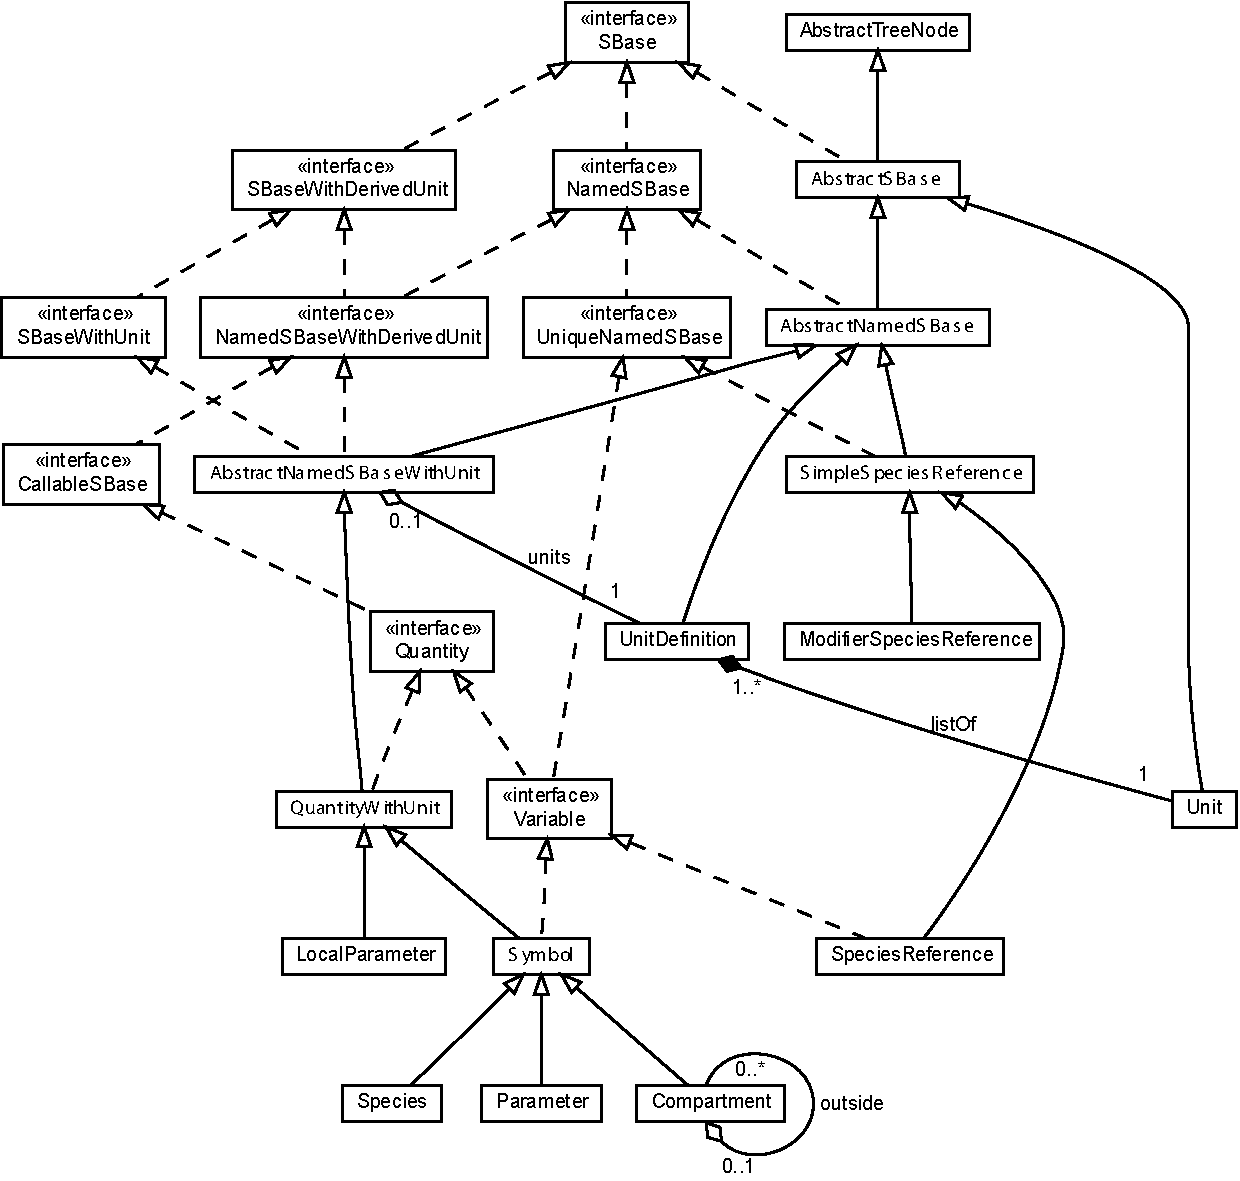
\includegraphics[width=\textwidth]{../common/img/Symbol.pdf}
  % Symbol.pdf: 596x587 pixel, 72dpi, 21.03x20.71 cm, bb=0 0 596 587
  \caption[The interface \Variable]{Part of JSBML's type
    hierarchy focusing on the interface \Variable.  In JSBML,
    those components of a model that may change their value during a
    simulation are referred to as \emph{variables}. The class \Symbol serves
    as the abstract superclass for variables that have units of measurement
    associated with them. Instances of \Parameter do not contain any
    additional fields. In \Species, a Boolean switch decides whether its
    value is to be interpreted as an initial amount or as an initial
    concentration. In contrast to \Variable{}s, \LocalParameter{}s represent
    constant unit-value pairs that can only be accessed within their
    declaring \KineticLaw. \index{SBML!variable}}
 \label{fig:Variable}
\end{figure}


If the SBML component can be addressed with an identifier (which means that
it has an \code{id} field in SBML), it will also implement the JSBML
interface \NamedSBaseWithDerivedUnit, and if it can appear within a formula
(which in JSBML, is represented using \ASTNode, discussed further below),
the entity will further implement the interface \CallableSBase, a special
case of \code{NamedSBaseWithDerivedUnit}.  When a component can be assigned
a unit explicitly, in JSBML the \SBaseWithUnit serves as its superclass.
JSBML further defines the convenience class \AbstractNamedSBaseWithUnit; it
extends \AbstractNamedSBase and implements interfaces \SBaseWithUnit
and \NamedSBaseWithDerivedUnit.  All elements derived from this abstract
class may, therefore, declare a unit and can be addressed using an
unambiguous SBML identifier.

In JSBML, the interface \Quantity describes an element that is associated
with a value, has at least a derived unit, and can be addressed using its
unambiguous identifier. JSBML uses the abstract class \QuantityWithUnit for
a \Quantity that explicitly declares its unit.  If the corresponding SBML
component includes a Boolean \index{Boolean} flag to indicate whether it is
a constant \index{SBML!constant} or a variable, JSBML
represents such a type using the interface \Variable.

SBML variables \index{SBML!variable} that have a defined unit are
represented as \Symbol objects.  (See \fig{fig:Variable}.) Thus,
the SBML elements \Compartment, \Parameter, and \Species are all special
cases of \Symbol in JSBML.  The specification of \SBMLthree introduced
another type of \Variable, which does not explicitly declare its unit:
\SpeciesReference.  Level~3 also introduced \LocalParameter, which is a
\QuantityWithUnit but not a \Variable because it is always constant.
\sec{sec:assignment-interface} explains the interfaces used for
changing the values of \Variable{}s.


\subsection{Interface for SBML components containing a mathematical
  formula: \codeNC{MathContainer}} 

The interface \MathContainer in JSBML gathers all those elements that may
contain mathematical expressions encoded in abstract syntax trees (i.e.,
instances of \ASTNode).  The abstract class \AbstractMathContainer serves
as actual superclass for the majority of the derived types.
\vrefrange{fig:MathContainer}{fig:MathContainerHierarchy} give a
better overview of how these data structures are organized and how they
relate to each other and other ones in JSBML.

\begin{figure}[hb]
 \centering
 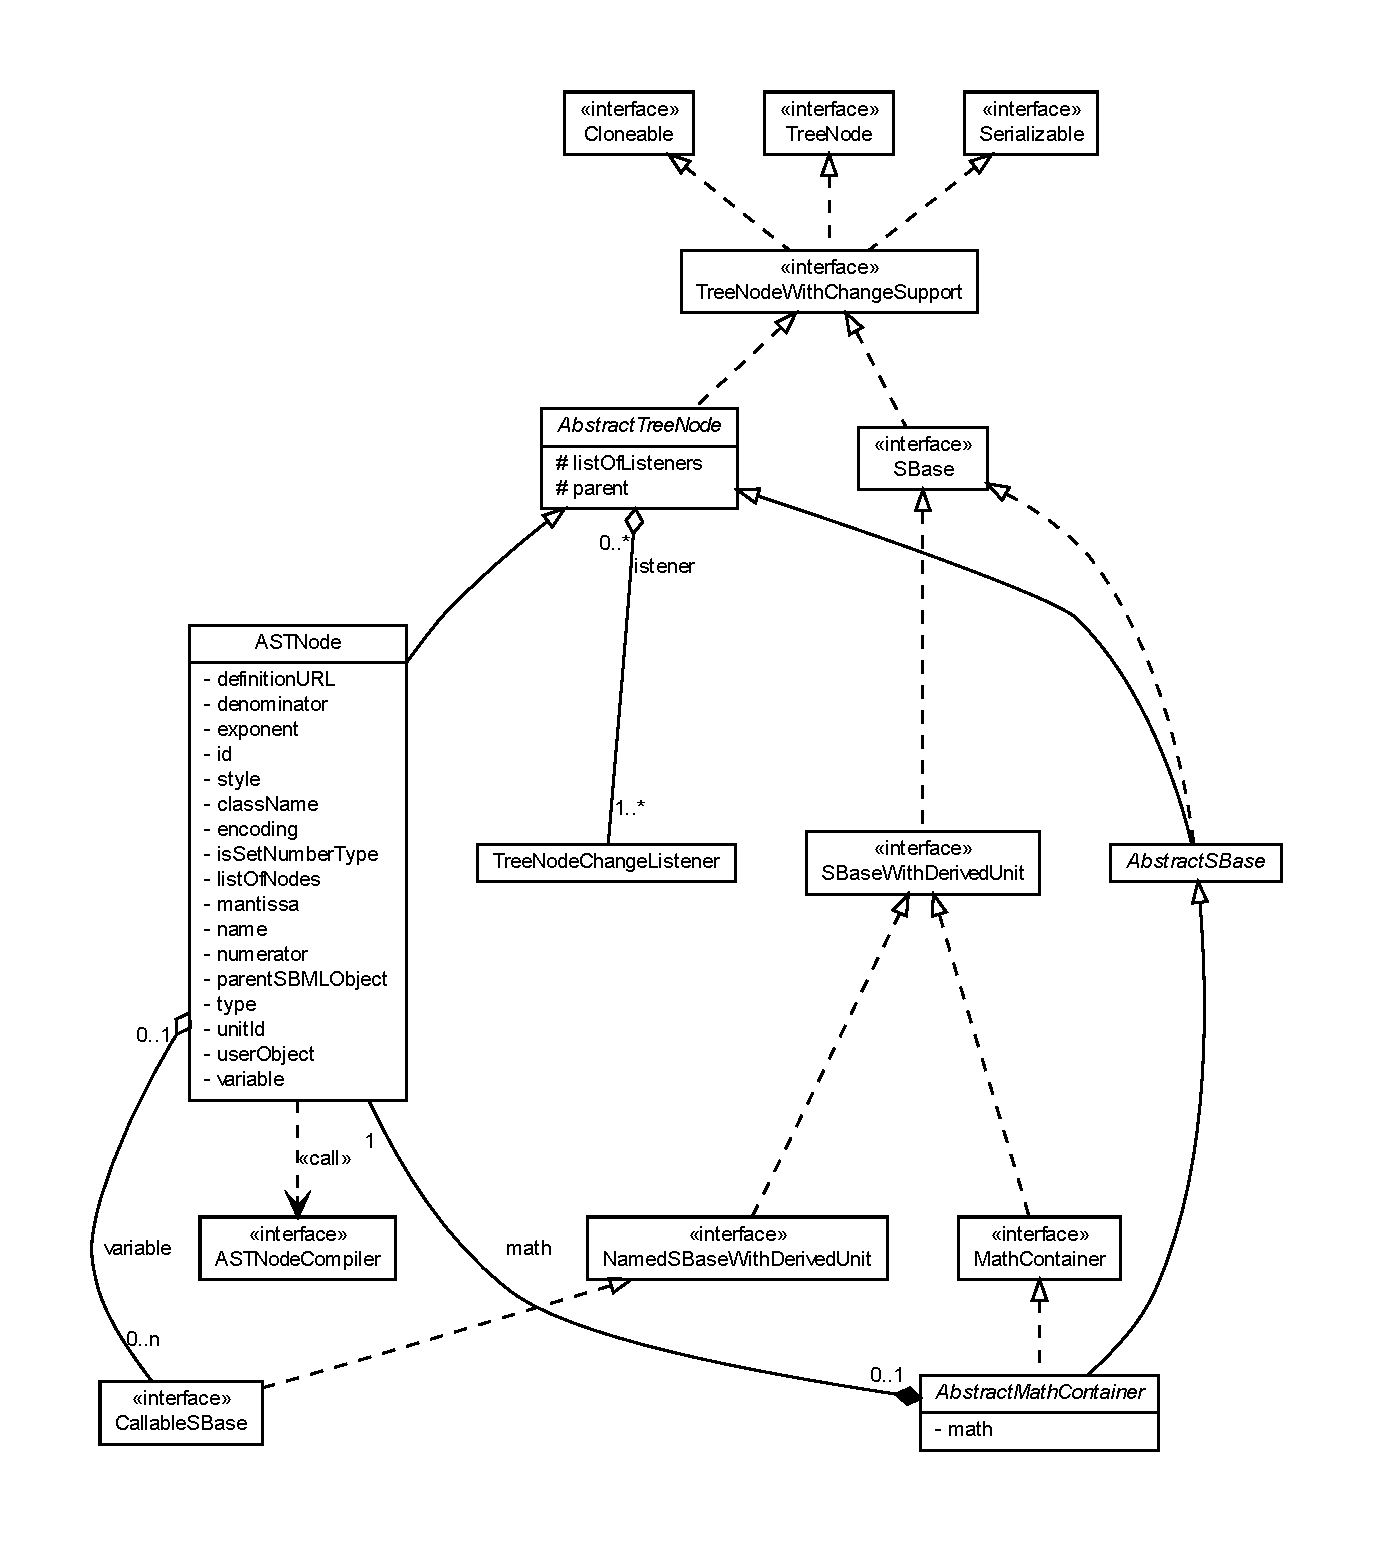
\includegraphics[width=\textwidth]{../common/img/ASTNode.pdf}
 % MathContainerClass.pdf: 557x396 pixel, 72dpi, 19.65x13.97 cm, bb=0 0 557 396
 \caption[Abstract syntax trees]{Abstract syntax trees (ASTs). The class
   \AbstractMathContainer serves as the superclass for several model
   components in JSBML. It provides methods to manipulate and access an
   instance of \ASTNode, which can be converted to or read from text
   strings containing formulas in a C-like infix syntax. Internally,
   \AbstractMathContainer{}s only deal with instances of \ASTNode. It
   should be noted that these abstract syntax trees do not implement the
   \SBase interface, but extend \AbstractTreeNode instead.}
 \label{fig:MathContainer}
\end{figure}

\begin{sidewaysfigure}
 \centering
 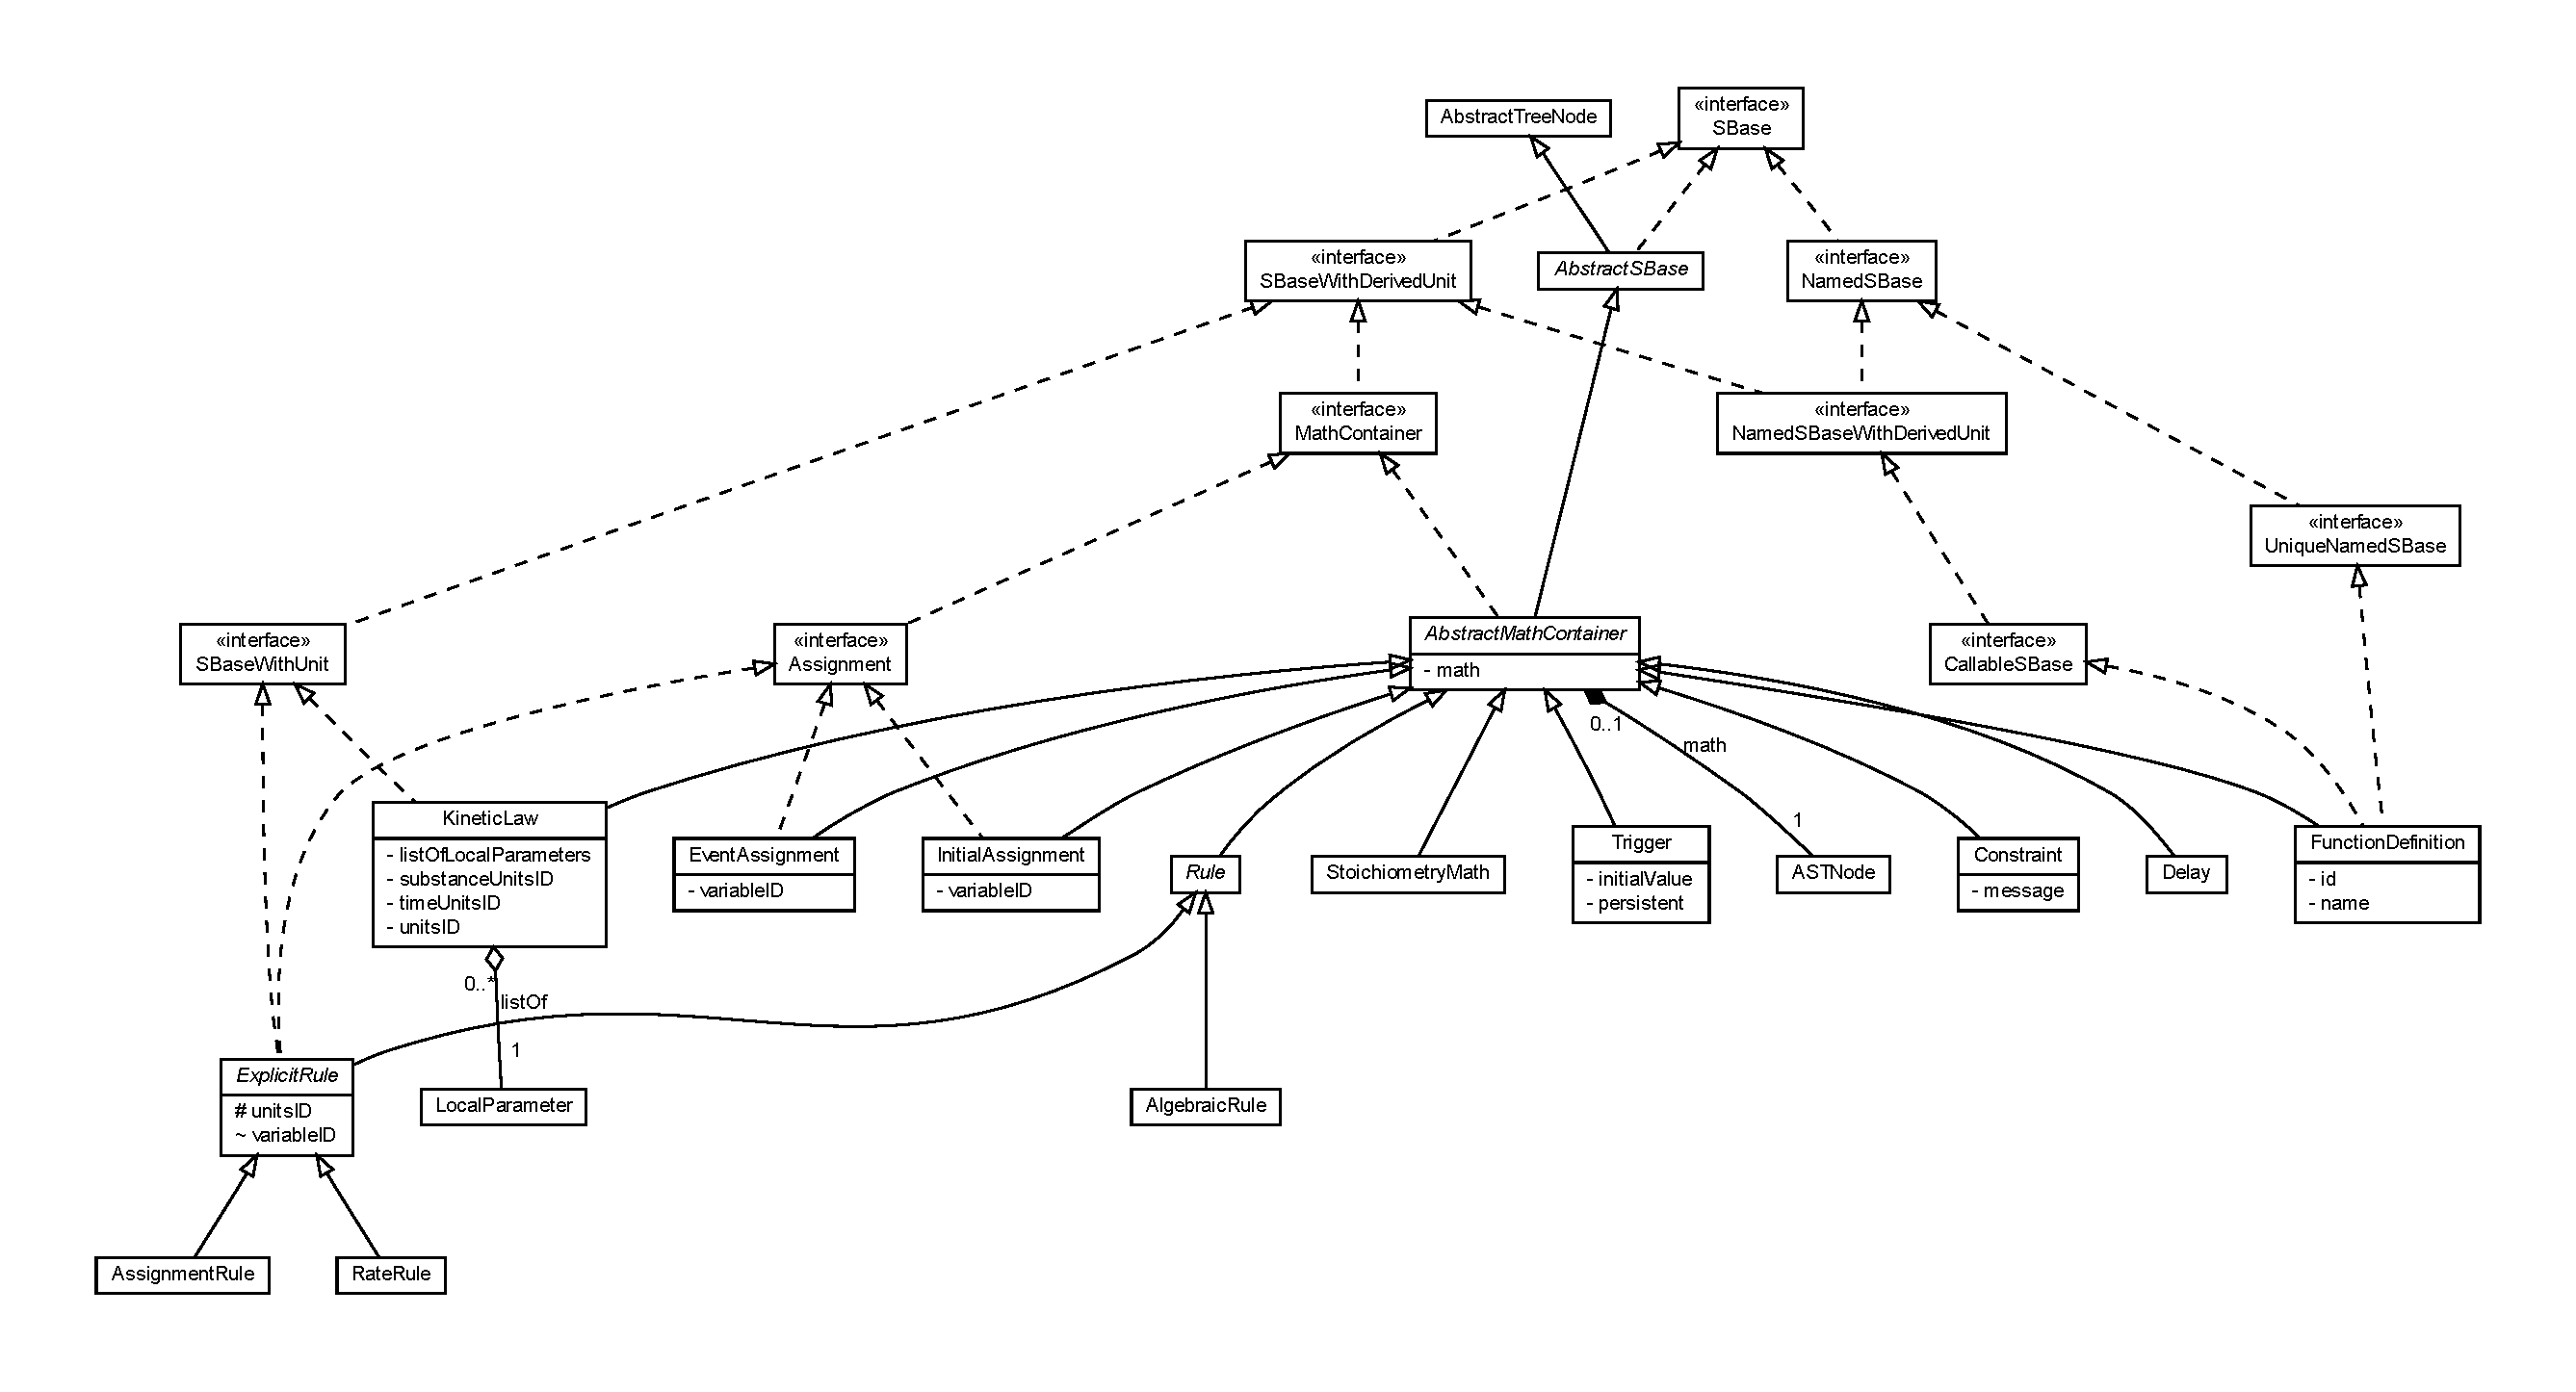
\includegraphics[width=\textwidth]{../common/img/MathContainer.pdf}
 % MathContainerClass.pdf: 557x396 pixel, 72dpi, 19.65x13.97 cm, bb=0 0 557 396
 \caption[Containers for mathematical expressions]{Containers for
   mathematical expressions. The interface \MathContainer, particularly its
   directly derived class \AbstractMathContainer, constitutes the
   superclass for all elements that store and manipulate mathematical
   formulas in JSBML.  The formulas themselves are stored in the form of
   \ASTNode objects. These can be evaluated using an implementation of
   \ASTNodeCompiler. Note that some classes that extend
   \AbstractMathContainer do not contain any of their own additional fields
   or methods.  This is the case for \Delay, \Priority, \StoichiometryMath,
   and \AlgebraicRule.}
 \label{fig:MathContainerHierarchy}
\end{sidewaysfigure}


\subsection{Interface for SBML components that may change the value of
  a variable: \codeNC{Assignment}}
\label{sec:assignment-interface}
\index{JSBML!assignment@\code{Assignment}}

JSBML provides a unified interface, \Assignment, for all objects that may
change the value of some variable in SBML. \index{SBML} This interface uses
the term \emph{variable} for the element whose value can be changed
depending on some mathematical expression that is also present in the
\Assignment (because the interface \Assignment extends the interface
\MathContainer).  Therefore, an \code{Assignment} contains methods such as
\code{set}-/\code{getVariable(Variable v)} and also \code{isSetVariable()}
as well as \code{unsetVariable()}.

In addition, JSBML also provides the methods
\code{set}-/\code{getSymbol(String symbol)} in the \InitialAssignment class
to make it easier to switch from libSBML to JSBML.  However, in JSBML, the
preferred way \index{JSBML!variable@\code{Variable}} is to apply the
methods \code{setVariable()}, either with \String or \Variable instances as
arguments.  \fig{fig:MathContainerHierarchy} shows the class
hierarchy surrounding the \Assignment interface in more detail.
